\documentclass[a4paper, 12pt, diplomski]{etfcyr}

\usepackage{fontspec}
\usepackage{polyglossia}
\usepackage[document]{ragged2e}
\usepackage{indentfirst}
\usepackage{enumitem}
\usepackage{scrextend}
\usepackage{etoolbox}
\usepackage{graphicx}
\usepackage{textcomp}
\usepackage{multicol}
\usepackage{float}
\usepackage{wrapfig}
\usepackage{listings}
\usepackage{array}

\DeclareGraphicsExtensions{.pdf,.png,.jpg}

\addtokomafont{labelinglabel}{\textbf}

\setdefaultlanguage[script=Cyrillic]{serbian}
\newfontfamily{\cyrillicfont}{Times New Roman}

\setmainfont{Times New Roman}
\setsansfont{Arial}
\setmonofont{PragmataPro}

\renewcommand*\contentsname{Садржај}

\newcommand{\indentfirstparagraphon}{
	\renewenvironment{justify}{%
		\trivlist
		\justifying
		\itemindent\JustifyingParindent
	\item\relax
	}{
		\endtrivlist
	}
}

\newcommand{\indentfirstparagraphoff}{
	\renewenvironment{justify}{%
		\trivlist
		\justifying
		\item\relax
	}{
		\endtrivlist
	}
}

\makeatletter
\gdef\tshortstack{\@ifnextchar[\@tshortstack{\@tshortstack[c]}}
\let\@tshortstack\@shortstack
\patchcmd\@tshortstack\vbox\vtop{}{}
\makeatother

\indentfirstparagraphon

\addto\captionsserbian{%
	\renewcommand{\bibname}%
	{Литература}%
}

\def\code#1{\texttt{#1}}
\def\quote#1{„#1“}

\lstset{basicstyle=\scriptsize\ttfamily,tabsize=4,frame=tb}

\setlength{\parindent}{4em}
\setlength{\JustifyingParindent}{4em}

\title{Паметна соба - контрола уласка}
\author{Топлица Танасковић}
\indeks{164/1996}
\date{септембар 2016.}
\mentor{Доц. др Саша Стојановић}
\predmet{Системско програмирање}

\begin{document}
	\sloppy
	\maketitle

	\thispagestyle{empty}
	\vspace*{\fill}
	\begin{center}
			\textit{\thanks{Овај рад посвећујем својим родитељима и супрузи која је имала разумевања и стрпљења за моју одсутност током рада на њему.}}
	\end{center}
	\vspace*{\fill}

	\begin{abstract}
		\begin{justify}
			У овом раду је изложен проблем прављења распореда коришћења лабораторија са контролом уласка. Објашњени су најчешћи сценарији који задају доста проблема и предложено је софтверско решење.
		\end{justify}
	\end{abstract}

	\begin{keywords}
		Дипломски радови, контрола приступа, програмирање, C++
	\end{keywords}
	\tableofcontents
	\listoffigures
	\listoftables

	\chapter{Увод}

		\section{Опис проблема}

		\begin{justify}
			Прављење распореда рада у факултетским лабораторијама је велики проблем са којим особље мора стално да се носи. Број студената и актвности које морају да се обаве је огроман, а факултет има ограничен број и лабораторија и радних места у њима. Ово представља проблем за људе који су одговорни за прављење распореда пошто морају да воде рачуна о много активности, студената и временских слотова док у исто време покушавају да избегну преклапања или конфликте.

			Проблем можемо сагледати са два аспекта, први је прављење распореда, а други је безбедност. Како је већ напоменуто, факултет има ограничен број лабораторија одређеног капацитета док је број студената са својим задацима и обавезним активностима огроман.

			Прављење распореда рада са дозволом уласка је врло тешко јер захтева праћење великог броја, како студената, тако и активности како би се обезбедило да нема преклапања. Радити ово ручно није оптимално и подложно је грешкама што може да доведе до разних преклапања, промена распореда у задњи час и многих других проблема. Без обзира што многе активности нису обавезне доста активности је у исто време и обавезно и врло битно за студенте, као што су рецимо колоквијуми или испити. Овакве активности не би смеле да се одлажу нити прекидају улажењем других особа у просторију.

			Што се тиче безбедности, неке лабораторије осим што имају деликатну и скупу, имају и врло опасну опрему која може услед погрешног руковања да начини огромну штету или чак нанесе опасне повреде. Због овога би требало ограничити приступ тј. улаз у неке од лабораторија како би се избегле у крајњим случајевима и несагледиве последице.
		\end{justify}

	\chapter{Дискусија}

		\section{Начини коришћења лабораторија}

			\begin{justify}
				Број начина на које једна лабораторија може да се користи углавном зависи од њене намене. Међутим, без обзира на намену лабораторије могу се уочити четири најчешћа начина на које се оне користе. Да би се целокупан проблем прецизније дефинисао, у овом одељку ће се дискутовати понаособ сваки од начина коришћења.
			\end{justify}

			\subsection{Дефиниције}

				\begin{justify}
					Пре него што будемо могли да опишемо начине на које се лабораторије користе, морамо увести неке дефиниције и успоставити релације између њих.
				\end{justify}

				\begin{labeling}{\smash{\tshortstack[l]{Корисник\\лабораторије}}}
					\indentfirstparagraphoff

					\item [Активност] 
						\begin{justify}
							Активност је било који процес који се одвија у лабораторији, без обзира на његово трајање, евентуалну периодичност или конкретан тип.
						\end{justify}

					\item[\smash{\tshortstack[l]{Тип\\активности}}]
						\begin{justify}
							Тип активности ближе дефинише активност, и одређује њен приоритет у односу на друге. Постоје следећи типови активности.
							\begin{enumerate}[noitemsep]
								\item Испит
								\item Колоквијум
								\item Предавања или вежбе
								\item Лабораторијске вежбе
								\item Посебни догађаји
								\item Индивидуални рад
							\end{enumerate}
						\end{justify}

					\item[\smash{\tshortstack[l]{Приоритет\\активности}}]
						\begin{justify}
							Приоритет активности одређује да ли је дозвољен улаз у просторију уколико се у њој преклапају активности, а једна од њих је битнија. Не желимо да допустимо да људи улазе и излазе из просторије док је у току испит. Приоритет активност је дефинисан типом активности како је наведено у претходној дефиницији.\\
							Индивидуални рад је посебан случај. Приликом заказивања такве активности може се посебно дозволити улазак без обзира на то да ли се у просторији већ одвија нека активност вишег приоритета. Ово се углавном користи за студенте који раде дипломски или неки други важан пројекат.
						\end{justify}

					\item[\smash{\tshortstack[l]{Корисник\\лабораторије}}]
						\begin{justify}
							Корисник лабораторије је било која особа којој се може дозволити улаз у лабораторију. Постоје две врсте корисника:
							\begin{enumerate}[noitemsep]
								\item Професор
								\item Студент
							\end{enumerate}
							Можда би се могао увести и студент демонстратор као засебан тип корисника, али како он нема посебна права, довољно је да буде члан листе која је маркирана као листа демонстратора како би могао да приступи лабораторији у заказаном термину без обзира да ли је нека друга активност у току.
						\end{justify}

					\item [Листа]
						\begin{justify}
							Листе су групе особа-корисника лабораторија које служе зарад лакше манипулације током заказивања активности и доделе права уласка у лабораторију. Постоје три врсте листи:
							\begin{enumerate}[noitemsep]
								\item Системске листе
								\item Трајне листе
								\item Привремене листе
							\end{enumerate}
							Привремене листе имају свој рок трајања и након тога се аутоматски бришу из система. Системске листе су посебан случај трајних листа, оне се не могу мењати и о њима систем сам води рачуна. Пример системске листе је листа студената друге године.
						\end{justify}

					\item [Просторија]
						\begin{justify}
							Просторија је било која лабораторија, кабинет или учионица у којој се одвијају неке активности у за коју желимо да имамо контролу уласка.
						\end{justify}

					\item[\smash{\tshortstack[l]{Системски\\корисник}}]
						\begin{justify}
							Системски корисници су особе које могу да врше подешавање система, имају контролу над свим подацима у систему и приступ извештају. Ови корисници су подељени у три улоге:
							\begin{enumerate}[noitemsep]
								\item Супер корисник
								\item Администратор
								\item Менаџер
							\end{enumerate}
							Шта је којој улози дозвољено да ради биће дефинисано касније када се буду дефинисале компоненте система.
						\end{justify}
					\indentfirstparagraphon
				\end{labeling}

			\subsection[Сценарио 1]{Испити и колоквијуми}
				\begin{justify}
				Ово је вероватно најбитнији сценариo. Активности дефинисане овим сценариом се обично не понављају и имају тачно дефинисан датум и време почетка као и трајање. Оваквим активностима се обично додељује искључиво једна листа студената, али није искључено да се доделе и више. Такође овакве активности се најчешће одвијају у више просторија паралелно
				\end{justify}

			\subsection[Сценарио 2]{Предавања или вежбе}
				\begin{justify}
					Предавања и вежбе су пример активности која се понавља на недељном нивоу један дужи временски период, и одвијају се у једној просторији. Ову врсту активности обично посећује иста група људи, прецизније студенти који слушају дати предмет или ако је предмет обавезан онда сви студенти дате године студија.
				\end{justify}

			\subsection[Сценарио 3]{Лабораторијске вежбе}
				\begin{justify}
					Лабораторијске вежбе су пример активности код којих поред студената и професора можемо имати и студенте демонстраторе. Студентима демонстраторима би требало такође дозволити несметан улаз и то се лако може постићи додавањем нове листе која ће садржати демонстраторе у систем, и додељивањем те листе активности. Овакве активности се најчешће изводе у једној просторији, али није немогуће да се одвијају паралелно у више.
				\end{justify}

			\newpage

			\subsection[Сценарио 4]{Посебни догађаји}
				\begin{justify}
					У овакве активност превасходно спадају јавна предавања, презентације и конференције. У оваквим случајевима у простиријама се увек налази неко од особља као што су предавачи, контрола приступа није потребна. Овакве активности не захтевају да имају додељену листу.
				\end{justify}

			\subsection[Сценарио 5]{Индивидуални рад}
				\begin{justify}
					Код ове врсте активност специфично је то што она може, ако је дефинисано, да дозволи улаз у просторију без обзира да ли је нека друга активност у току. Оваква активност захтева листу студената, којој може да припада и само један студент. Овакве активности се најчешће одобравају студентима који раде дипломски или неки други важан рад, а имају потребу за опремом која се налази у лабораторијама.
				\end{justify}

		\section{Посебне напомене}
			\begin{justify}
				Уколико је неопходно, могуће је одређеним студентима забранити улазак у неку просторију. Студенти којима је улаз забрањен неће моћи да уђу у дату просторију иако су на листи за активност која се одвија у њој.
			\end{justify}

	\chapter{Предлог решења}

		\section{Уопштени преглед система}
			\begin{justify}
				Услед саме природе проблема, као и потребе да компоненте комуницирају на поуздан и безбедан начин, систем мора да буде модуларан са прецизно дефинисаним протколима комуникације и обраде грешака. Уопштен дијаграм система дат је на слици испод.

				\begin{figure}[h]
					\begin{center}
						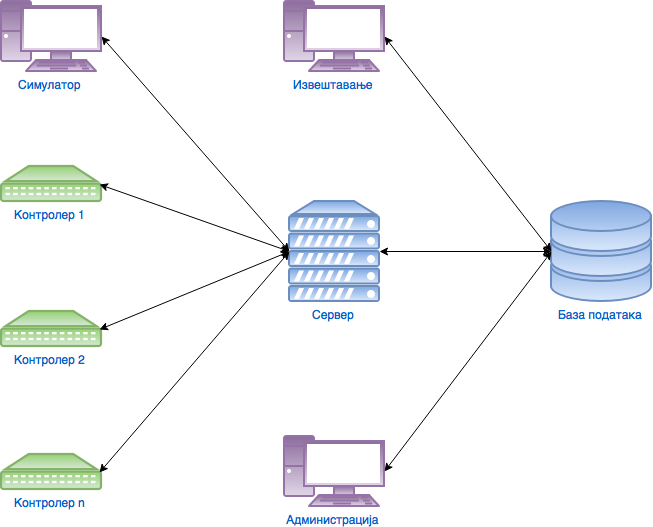
\includegraphics[scale=0.47]{SystemOverview.png}
					\end{center}
					\caption{Дијаграм система}
					\label{figure:1}
				\end{figure}

				Са дијаграма на слици \ref{figure:1} лако можемо уочити да постоје три различите врсте компоненти. Плаве су чисто софтверске компоненте које раде на серверу, љубичасте су такође софтверске компоненте, али раде на локалним рачунарима, док су зелене компоненте представљају микроконтролере са припадајућом хардверсо-софтверском подршком.
			\end{justify}

		\section{Компоненте система}

			\subsection{База података}
				\begin{justify}
					Сервер базе података је одговоран за свеобухватно похрањивање података. Посебних хардверских захтева нема, сем да постоји довољно меморије и складишног простора на диску. Сервер базе података који се користи у овом решењу је PostgreSQL издање 9.2, а може се користити и новија верзија.
					\begin{figure}[h]
						\begin{center}
							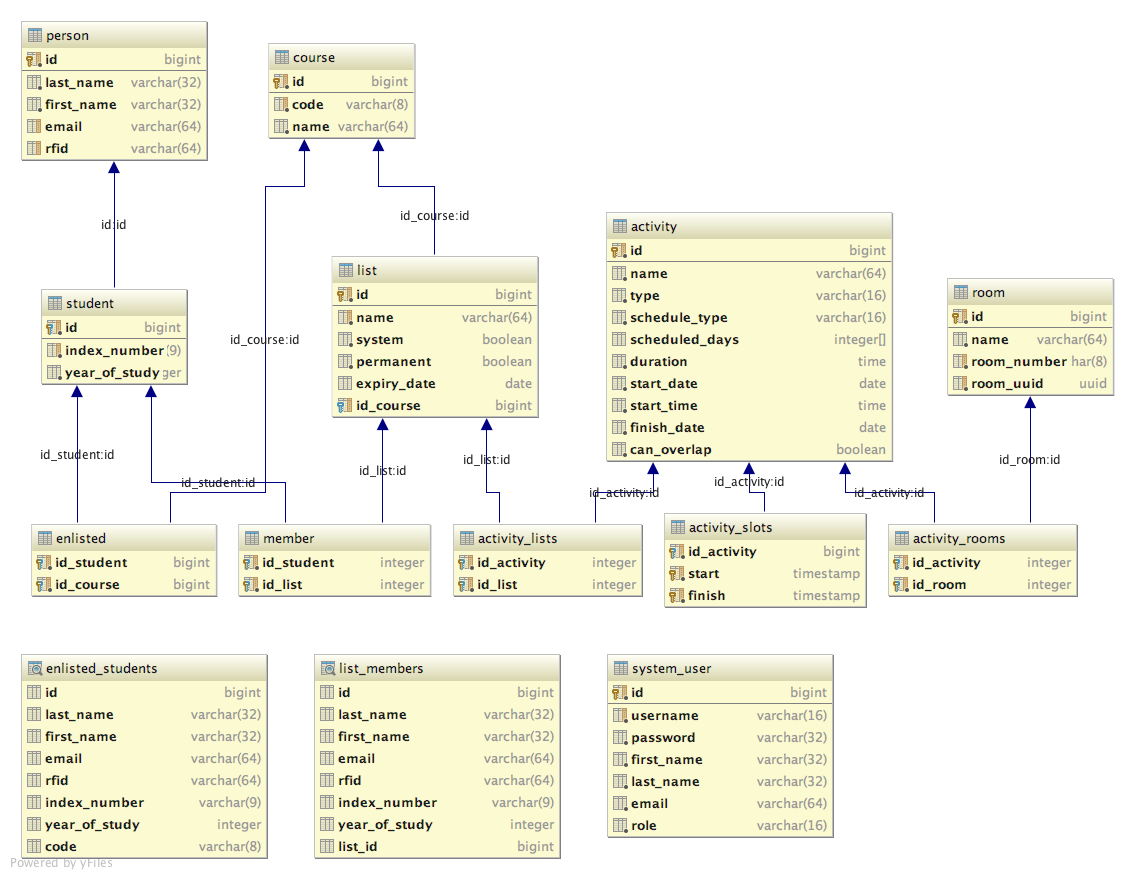
\includegraphics[scale=0.25]{DatabaseDiagram.png}
						\end{center}
						\caption{Дијаграм базе података}
						\label{figure:2}
					\end{figure}
				\end{justify}
				
			\subsection{ПаСо Сервер}
				\begin{justify}
					ПаСо сервер је централна компонента система. Његова одговорност је да комуницира са контролерима просторија и са симулатором као алатом за тестирање. Сам сервер је имплементиран као стандардни UNIX димон који прихвата TCP конекције на порту који је одређен подешавањима. Овај сервер није пасивна компонента која само чека захтеве и обрађује их, већ периодично шаље и ”јеси ли жив” сигнале пријављеним контролерима и симулаторима. Такође, одговоран је и за слање података које би контролери требало да користе уколико дође до прекида у комуникацији. Формат комуникације, порука и података за случај прекида саме комуникације биће дефинисан касније.
					Илустрација рада сервера дата је на слици \ref{figure:3}.
					\begin{figure}[h]
						\begin{center}
							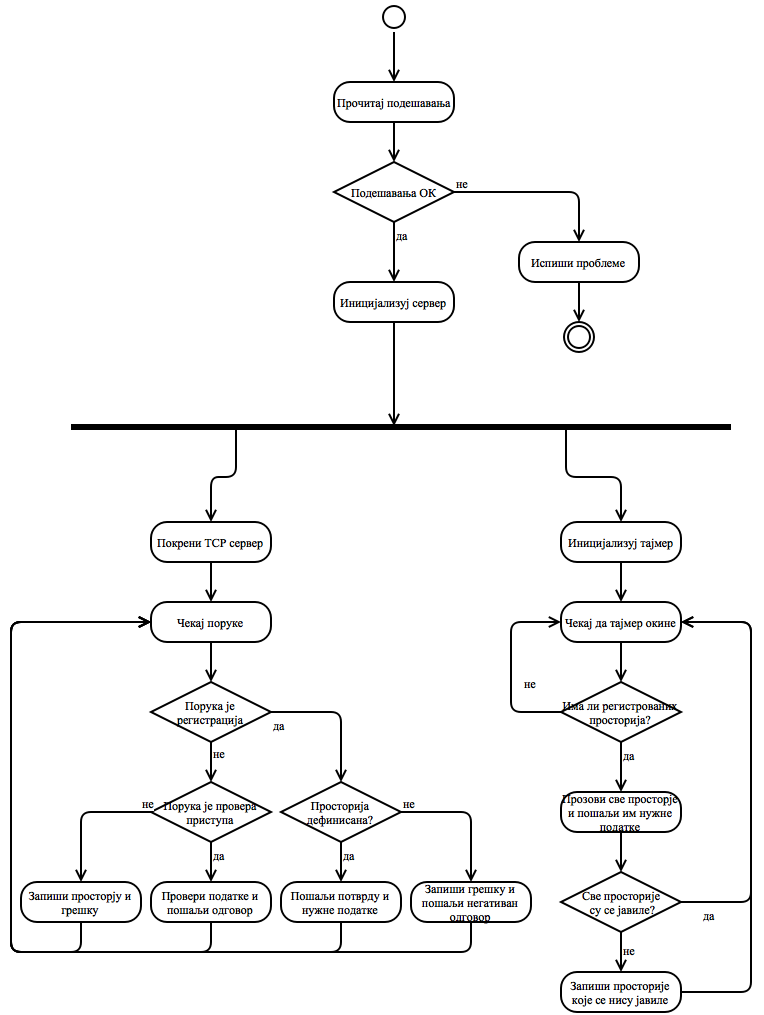
\includegraphics[scale=0.35]{ServerWorkflow.png}
						\end{center}
						\caption{Дијаграм рада сервера}
						\label{figure:3}
					\end{figure}
				\end{justify}

			\subsection{Администрација}
				\begin{justify}
					Ова компонента је одговорна за комплетну администрацију целог система, почев од управљања корисницима и просторијама па све до заказивања активности. У администравном програму постоје следећи модули:

					\begin{labeling}{\smash{\tshortstack[l]{Управљање\\активностима}}}
						\indentfirstparagraphoff

						\item[\smash{\tshortstack[l]{Управљање\\системским\\корисницима}}]
							\begin{justify}
								Овај модул служи за одржавање листе корисника система. Корисници дефинисани у овом модулу немају никаве везе са корисницима лабораторија и служе искључиво за администрацију система. Сви корисници су распоређени у више улога, о чему ће бити речи касније.
							\end{justify}

						\item[\smash{\tshortstack[l]{Управљање\\просторијама}}]
							\begin{justify}
								Поред уношења нових просторија и дедељивања јединственог идентификатора, управљање просторијама подразумева и одржавање листе студената којима је забрањен улаз за сваку просторију понаособ.
							\end{justify}

						\item[\smash{\tshortstack[l]{Управљање\\предметима}}]
							\begin{justify}
								Овај део се бави одржавањем података о предметима на факултету и подржава увоз како података из CSV датотека. Постоје две врсте података које се могу увозити. Прва врста је сама листа предмета са припадајућим подацима, а друга је представља податке о студентима који слушају одређени предмет. Формати CSV датотека за обе врсте података биће дати касније у засебном одељку.
							\end{justify}

						\item[\smash{\tshortstack[l]{Управљање\\студентима}}]
							\begin{justify}
								Овај модул служи за одржавање комплетне листе студената. Поред стандарних података о студенту као што је број индекса, име и презиме, електронска пошта итд. у овом модулу се уноси и РФИД студентских картица које омогућавају студентима приступ факултетским просторијама. Уколико је потребно студенту забранити приступ свим просторијама где се врши контрола уласка, довољно је само обрисати РФИД из његовиг личних података и он више неће моћи својом картицу да користи за откључавање врата.
								За сваког студента се могу видети детаљи као што су подаци о томе које предмете слуша и којих је листа члан.
								Као и претходни модул, и овај подржава увоз података о студентима из CSV датотека.
							\end{justify}

						\newpage

						\item[\smash{\tshortstack[l]{Управљање\\наставним\\особљем}}]
							\begin{justify}
								Управљање наставним особљем је у суштини исто као и управљање студентима, са разликом што наставно особље не припада ни једној листи, већ се њима увек дозвољава улазак у просторије без обзира да ли се нека активност одвија или не. Наравно, и овде је довољно обрисати РФИД из података да би се онемогућио улазак у просторије се контролом приступа. Ово је згодно уколико дође до губљења или крађе картице.
							\end{justify}

						\item[\smash{\tshortstack[l]{Управљање\\листама}}]
							\begin{justify}
								Сврха овог дела је да пружи решење за лакшу манипулацију правима приступа, као и за лакшу прегледност груписањем студената у листе. Такође, обезбеђен је и увоз података у виду чланова за сваку листу. Када су у питању системске листе, њихова измена, нити брисање није могуће пошто о њима бригу води сам систем.
							\end{justify}

						\item[\smash{\tshortstack[l]{Управљање\\активностима}}]
							\begin{justify}
								Ово је најкомплекснији и вероватно најбитнији део администрације, пошто се поред креирања активности бави и њиховим заказивањем које може бити различито у зависности од потребе. Свака активност садржи мноштво података те се зарад боље прегледности уређивање одвија у корацима путем чаробњака. Што се тиче заказивања активности подржана су два начина, заказивање једног тачно одређеног термина, и заказивање на одређени временски период са понављањем на недељном или месечном нивоу. У оба случаја где се активност понавља потребно је одабрати тачне дане понављања у недељи или месецу.
							\end{justify}

						\end{labeling}
				\end{justify}

			\newpage

			\subsection{Приступ модулима у зависности од системске улоге}
				\begin{justify}
					Матрица приступа административном модулу у зависности од улoге додељеном системском кориснику дата је у табели \ref{table:1}.
				\end{justify}
				\begin{table}[H]
					\centering
					\begin{tabular}{ c||c|c|c }
						Модул\textbackslash Улога & Супер корисник & Администратор & Менаџер \\
						\hline\hline
						Системски корисници & да & да & не \\
						Просторије & да & да & не \\
						Предметими & да & не & да \\
						Студенти & да & не & да \\
						Наставници & да & не & да \\
						Листе & да & не & да \\
						Активности & да & не & да \\
						\hline
					\end{tabular}
					\caption{Приступ модулима у зависности од системске улоге}
					\label{table:1}
				\end{table}

			\subsection{Извештавање}
				\begin{justify}
					Компонента задужена за извештавање не постоји као физички засебна компонента система, већ је интегрисана у административни модул. Понуђена су три извештаја, два се односе на безбедност, то је извештај улазака у одабрану просторију и сви уласци одређене особе у било коју од просторија, док трећи даје преглед заузећа собе. Извештаји везани за просторије се налазе у одељку за управљање просторијама, док се извештај за о уласцима особа у просторија налазе у одељцима за управљање студентима односни наставним особљем.
				\end{justify}

			\subsection{Контролери просторија}
				\begin{justify}
					Ова компонента са припадајућим хардвером и софтвером служи да контролише аутоматску браву на вратима просторија, чита РФИД картице или токене и комуницира са сервером.
					Сваки контролер, пре него што може да се стави у употребу мора да се подеси и да се одговарајућа просторија унесе у систем путем административног модула. Подешавање подразумева да се у контролер унесе јединствени идентификатор собе који је административни модул изгенерисао, као и адреса ПаСо сервера.
				\end{justify}

				\subsubsection*{Опис рада контролера просторије}

					\begin{figure}[h]
						\begin{center}
							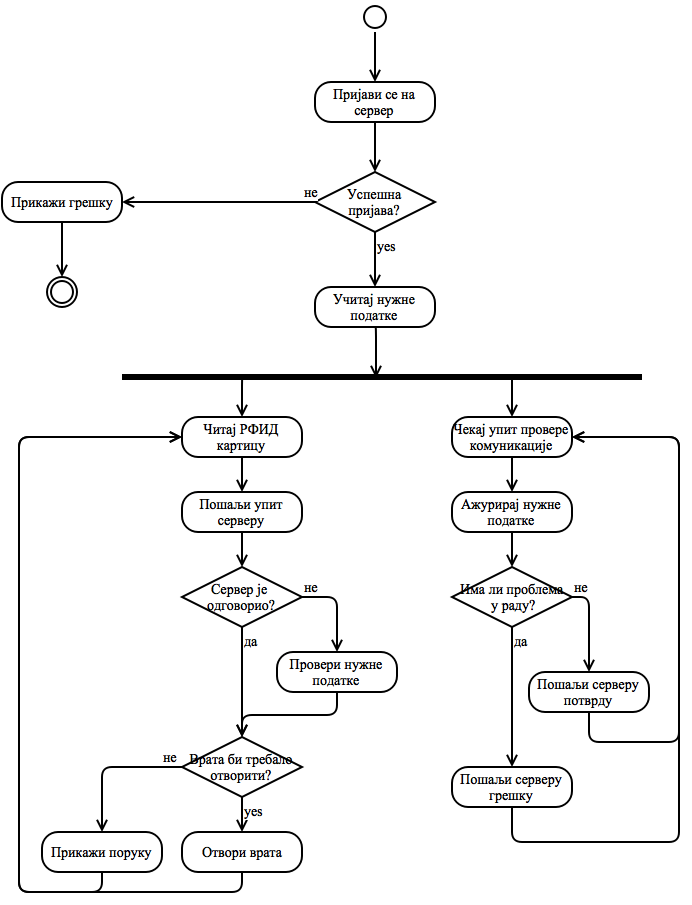
\includegraphics[scale=0.4]{RoomControllerWorkflow.png}
						\end{center}
						\caption{Дијаграм рада контролера}
						\label{figure:4}
					\end{figure}
					\begin{justify}
						Као што се може видети на слици \ref{figure:4}, по укључивању напајања, контролер би требало да се региструје на сервер. Ово је неопходно из разлога што сервер мора да зна адресу контролера како би могао периодично да шаље захтеве којима ће да проверава да ли комуникација са контролером није случајно прекинута. Поред захтева којима се проверава стање комуникације, сервер мора периодично да шаље контролеру податке који су му неопходни за рад уколико до прекида комуникације ипак дође. Ови подаци не представљају ништа друго до РФ идентификатора картица и токена наставног особља, како би у случају да нема комуникације они могли несметано да улазе у просторије или отворили врата особљу задоженом за одржавање опреме.
						Након регистрације, контролер чека на читање РФИД картице или токена, након чега шаље серверу упит да ли би требало да отвори врата датој особи. Паралелно са тим контролер слуша на TCP како би могао да одговори на серверове провере стања комуникације и прихвати податке за рад у случају прекида исте. Детаљан формат комуникације између сервера и контролера биће дат у засебном одељку.
					\end{justify}

			\subsection{Симулатор}
				\begin{justify}
					Симулатор је компонента чија сврха је да убрза развој и потпомогне тестирање како сервера тако и контролера просторија. Такође, може се користити и за проверу понашања система под различитим околностима. Симулатор је написан као класична интерактивна десктоп апликација и има исти алгоритам рада као и контролер просторије. Главна улога симулатора, поред тестирања сервера, јесте да особама које раде на развоју хардверских контролера просторија да увид у формат и протокол комуникације, како обрађивати грешке, итд. Све поруке које се размењују између симулатора и сервера могу се видети директно у самом симулатору користећи JSON нотацију. Поред симулације читања РФИД картица и токена, компонента може да симулира и прекид комуникације са сервером.
				\end{justify}

		\newpage

		\section{Протокол комуникације и формати порука}
			\begin{justify}
				Због лакшег развоја и отклањања проблема, како у току развоја тако и за време експлоатације система, све поруке које се размењују између компоненти су у JSON формату.
			\end{justify}

			\subsection{Безбедност комуникације}
				\begin{justify}
					Да би се повећала безбедност система и спречило било какво ослушкивање саобраћаја сва комуникација је осигурана TLSv10 SSL протоколом.
				\end{justify}
			
			\subsection{Основни формат поруке}
				\begin{justify}
					Свака порука која се шаље, на почетку увек има два бајта која означавају њену дужину, а након њих следи сама порука у JSON формату. Дужина прослеђена у прва два бајта не укључује та два бајта, и уколико се послата дужина поруке и њена стварна-прочитана дужина не слажу, порука ће се сматрати неисправном и биће игнорисана. Све поруке које долазе од контролера или симулатора морају да имају \quote{room-id} и \quote{operation} поља уз додатак других ако је то неопходно. Сваки одговор на поруку мора имати исту вредност у пољу \quote{operation}.
					За опис свих порука користи се \quote{JSON Schema} формат о коме се може прочитати са следеће интернет странице http://json-schema.org.
				\end{justify}

			\newpage

			\subsection{Регистрација контролера или симулатора на сервер}
				\begin{justify}
					Поруке које контролери или симулатори шаљу да би се регистровали на систем морају да одговарају следећој JSON шеми:
					\begin{lstlisting}
{
	"$schema": "http://json­schema.org/draft­04/schema#",
	"description": "The room registration request",
	"type": "object",
	"properties": {
		"room­id": { "type": "string" },
		"operation": { "type": "string" }
	},
	"required" : ["room­id", "operation"]
}
					\end{lstlisting}
					Вредност поља \quote{operation} за поруке регистрације на сервер је увек \quote{register}.
					Очекиван одговор од сервера је у следећем формату:
					\begin{lstlisting}
{
	"$schema": "http://json­schema.org/draft­04/schema#",
	"description": "The room registration response",
	"type": "object",
	"properties": {
	"room­id": { "type": "string" },
	"operation": { "type": "string" },
	"success": { "type": "boolean" },
	"port": { "type": "integer" },
	"emergency­data" : {
		"type": "array",
		"items": { "type": "string" }
		}
	}
	"required": [ "room­id", "operation", "success" ]
}
					\end{lstlisting}
				\end{justify}

			\newpage

			\subsection{Провера комуникације и статуса контролера}
				\begin{justify}
					Ове поруке шаље сервер како би проверио да комуникација није прекинта, као и да добије повратну информацију од контролера о његовом стању. Формат ове поруке је следећи:
					\begin{lstlisting}
{ 
	"$schema": "http://json­schema.org/draft­04/schema#",
	"description": "Are you alive request",
	"type": "object",
	"properties": {
		"room­id": { "type": "string" },
		"operation": { "type": "string" },
		"emergency­data" : {
			"type": "array",
			"items": { "type": "string" }
		}
	}
	"required": [ "room­id", "operation" ]
}
					\end{lstlisting}
					Вредност поља \quote{operation} је увек \quote{ping}.
					Очекивани одговор од контролера или симулатора је следећи:
					\begin{lstlisting}
{
	"$schema": "http://json­schema.org/draft­04/schema#",
	"description": "Are you alive response",
	"type": "object",
	"properties": {
		"room­id": { "type": "string" },
			"operation": { "type": "string" },
			"response": { "type": "boolean" },
			"fault": { "type": "string" }
		}
	"required": [ "room­id", "operation", "response" ]
}
					\end{lstlisting}
					Вредност поља \quote{response} може да буде \quote{false}, у том случају у мора постојати и поље \quote{fault} које садржи разлог отказа контролера, на пример, неисправан хардвер, и сервер ће уписати ту поруку у свој дневник. У случају да је све уреду поље \quote{response} има вредност \quote{true} и поље \quote{fault} није обавезно.
				\end{justify}

			\newpage

			\subsection{Провера права приступа}
				\begin{justify}
					Ову поруку шаље контролер по очитавању картице да би са сервером проверио да ли би особу требало пустити у просторију. Формат је следећи:
					\begin{lstlisting}
{
	"$schema": "http://json­schema.org/draft­04/schema#",
	"description": "The access permission query",
	"type": "object",
		"properties": {
			"room­id": { "type": "string" },
			"operation": { "type": "string" },
			"rfid" : { "type": "string" }
		}
	"required": [ "room­id", "operation", "rfid" ]
}
					\end{lstlisting}
					Поље \quote{operation} је \quote{access}. Одговор је у следећем формату:
					\begin{lstlisting}
{
	"$schema": "http://json­schema.org/draft­04/schema#",
	"description": "The access permission query response",
	"type": "object",
		"properties": {
			"room­id": { "type": "string" },
			"operation": { "type": "string" },
			"granted" : { "type": "boolean" }
		}
	"required": [ "room­id", "operation", "granted" ]
}
					\end{lstlisting}
					Уколико вредност поља \quote{granted} није \quote{true} контролер неће отворити-откључати врата.
				\end{justify}

		\section{Увоз и извоз података}
			\begin{justify}
				За увоз и извоз података користи се искључиво CSV формат. Структура CSV датотеке мора у потпуности да одговара форматима који су дефинисани у овом одељку, несмеју садржати празне редове нити било какве друге податке. Подаци који се могу увозити су:
				\begin{enumerate}[noitemsep]
					\item Подаци о предметима.
					\item Подаци о студентима.
					\item Листе студената који слушају одређени предмет.
					\item Произвољне листе студената, као на пример списак за полагање испита.
				\end{enumerate}
				Подаци који се могу извозити су извештаји и то:
				\begin{enumerate}[noitemsep]
					\item Списак особа које су улазиле у одређену просторију у датом периоду.
					\item Списак просторија у које је одређена особа улазила у датом периоду.
					\item Извештај о заузећу одабране просторије.
				\end{enumerate}
			\end{justify}

			\subsection{Формат података за увоз}
				\begin{justify}
					Формат CSV датотека које представљају списак студената који слушају неки предмет, или рецимо списак за лабораторијске вежбе или испит је у потпуности произвољан уз ограничење да број индекса мора стајати на почетку, остатак реда се игнорише.
					Формати датотека за увоз осталих подржаних података су дати у табелама испод.
				\end{justify}
				\begin{table}[H]
					\centering
					\begin{tabular}{ c|c|c }
						Колона & Значење & Тип \\
						\hline\hline
						1. & шифра предмета & текст \\
						2. & име предмета & текст \\
						\hline
					\end{tabular}
					\caption{Формат за увоз података о предметима}
					\label{table:2}
				\end{table}
				\begin{table}[H]
					\centering
					\begin{tabular}{ c|c|c }
						Колона & Значење & Тип \\
						\hline\hline
						1. & име & текст \\
						2. & презиме & текст \\
						3. & ел. пошта & текст \\
						4. & број индекса у формату гггг/бббб & текст \\
						5. & година студија & цео број \\
						\hline
					\end{tabular}
					\caption{Формат за увоз података о студентима}
					\label{table:3}
				\end{table}

			\newpage

			\subsection{Формат за извоз података}
				\begin{justify}
					Извештаји о уласцима особа у одређену просторију или улазасцима одређене особе за неки период су идентични у свом фомату и дати су у табели \ref{table:4}, док је формат извештаја о заузећу неке просторије дат у табели \ref{table:5}.
					\begin{table}[H]
						\centering
						\begin{tabular}{ c|c|c }
							Колона & Значење & Тип \\
							\hline\hline
							1. & број просторије & текст \\
							2. & број индекса или интерни број запосленог & текст \\
							3. & име & текст \\
							4. & презиме & текст \\
							5. & датум и време & ИСО 8061 формат \\
							\hline
						\end{tabular}
						\caption{Формат извештаја о уласцима}
						\label{table:4}
					\end{table}
					\begin{table}[H]
						\centering
						\begin{tabular}{ c|c|c }
							Колона & Значење & Тип \\
							\hline\hline
							1. & број просторије & текст \\
							2. & активност која је у питању & текст \\
							3. & почетак активности & ИСО 8061 формат \\
							4. & крај активности & ИСО 8061 формат \\
							\hline
						\end{tabular}
						\caption{Формат извештаја о заузећу просторије}
						\label{table:5}
					\end{table}
					Извештај о заузећу неке простије може бити користан као распоред који би стајао на вратима како би студенти и наставници знали кад се шта одвија у њој.
				\end{justify}

		\section{Опоравак система од проблема}
			\begin{justify}
				У овом систем може доћи два велика проблема. Први је физички отказ контролера који управља просторијом. У зависности колико је озбиљан проблем, контролер може у потпуности престати са радом, тако да неће моћи да одговара на периодичне провере комуникације инициране од стране сервера. Уколико сервер не добије одговор записаће проблем у дневник. Ако, пак, контролер може да одговара на провере комуникације требало би, у том случају, у свом одговору у пољу \quote{response} да пошаље \quote{false} и да у пољу \quote{fault} проследи опис грешке. Нажалост, код оваквих отказа систем не може пуно тога да уради, осим да обавести одржавање или обезбеђење о проблему. У овој имплементацији информација о отказу је само записана у дневник.

				Други проблем је прекид канала комуникацији услед, рецимо, покиданог мрежног кабла или бежичног рутера који је престао да ради. У овом случају контролер ће прећи у режим рада са последњим приљеним нужним подацима, што значи да ће само наставно особље моћи да отвара врата просторије. У нади да ће успоставити комуникацију контролер ће наставити да покушава да пошаље поруке приликом сваког очитавања РФИД картице или токена. Са друге стране, сервер ће открити да контролер не одговара на провере комуникације и убележиће догађај у дневник. Оног тренутка када се канал комуникације поново успостави обе компоненте ће наставити да раде као да се ништа није ни догодило.
			\end{justify}

		\section{Напомене о имплементацији}
			\begin{justify}
				У овом раду израђене су све наведене компоненте система, осим физичких контролера просторија који су остављени за евентуално будуће проширење или наставак овог рада. Софтверске компоненте су написане C++ програмским језиком уз коришћење C++11 стандарда и требало би да раде без икаквих измена било којој модерној Linux или UNIX дистрибуцији. Цео систем је развијан и детаљно тестиран само на линукс дистрибуцијама Ubuntu 16.04 и CentOS 7, уз коришћење PostgreSQL базе података минималне верзије 9.2. Windows оперативни систем није подржан. Кратка упутства за компајлирање, инсталацију и подешавање система дата су у одговарајућим README датотекама у оквиру изворног кода.
			\end{justify}

	\chapter{Инсталација и подешавање}

		\section{Потребан софтвер}

		\section{Компајлирање и инсталација}

		\section{Подешавање}

	\chapter{Корисничко упутство}

		\section{Сервер}

		\section{Административна конзола}

		\section{Симулатор}


	\begin{thebibliography}{9}
		\bibitem{qt_website}
		The Qt Company, \quote{Qt Documentation},
		http://doc.qt.io

		\bibitem{cplusplus}
		cplusplus.com, \quote{C++ Reference},
		http://www.cplusplus.com/reference

		\bibitem{postgresql}
		PostgreSQL, \quote{Documentation},
		https://www.postgresql.org/docs

		\bibitem{jsonschema}
		JSON Schema and Hyper-Schema, \quote{Documentation},
		http://json-schema.org/documentation.html

		\bibitem{pragprog}
		Andrew Hunt, David Thomas, \quote{The Pragmatic Programmer: From Journeyman to Master},
		прво издање, The Pragmatic Bookshelf, 1999, ИСБН 978-0-2016-1622-4
		
		\bibitem{tddcpp}
		Jeff Langr, \quote{Modern C++ Programming with Test-Driven Development: Code Better, Sleep Better},
		прво издање, The Pragmatic Bookshelf, 2013, ИСБН 978-1-937785-48-2
	\end{thebibliography}
\end{document}